\newpage
\subsection*{Обработка данных}


В логарифмическом масштабе построим $\ln(U \times  I)[\ln(\sub{t}{surf})]$. Начиная с температуры $\sub{t}{surf} \sim 1500 \celc$ (красная точка на графике) вольфрамовая нить светилась почти полностью, начиная с этой температуры приближаем из соображений
\begin{equation*}
    UI = W = \varepsilon_T B T^n, 
    \hspace{0.5cm} \Rightarrow \hspace{0.5cm}
    \ln W = \ln(\varepsilon_T B) + n \ln (T).
\end{equation*}
Лабораторный практикум предлагает игнорировать зависимость $\varepsilon_T (\sub{t}{surf})$, однако это вносит достаточно существенные изменения, поэтому данные из таблицы лабораторного пракикума (таблица №1, стр. 236) восттановили зависимость $\varepsilon_T (T)$.  
\vspace{-5mm}

\begin{figure}[h]
    \centering
    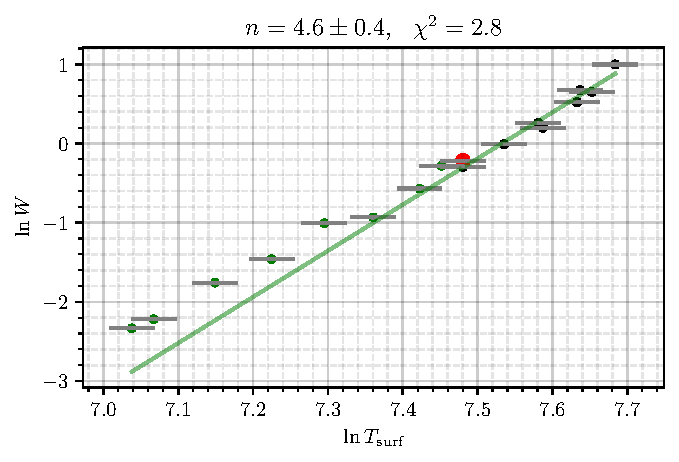
\includegraphics[width=0.6\textwidth]{figs/fig2.pdf}
    \vspace{-5mm}
    \caption{Приближение зависимости $W(\sub{t}{surf})$}
    \label{fig:plot}
\end{figure}


Значения $\chi^2 = 2.8$ говорит об адекватности приближения в рамках данной погрешности. 
Итого, находим значение для $n$
\begin{equation*}
    n = 4.8 \pm 0.4,
\end{equation*}
что, учетом погрешности, сходится с ожиданиями. 

Теперь определим постоянную Стефана-Бльцмана. Основной вклад в погрешность даёт температура в силу $T^4$. Также наблюдается постоянный сдвиг, скорее всего связанный с неточностью указанной $S = 0.36 \text{ см}^2$, измерить которую не представляется возможным (значение лучше сходится с табличным при $S = 0.27 \text{ см}^2$). 

\begin{figure}[h]
    \centering
    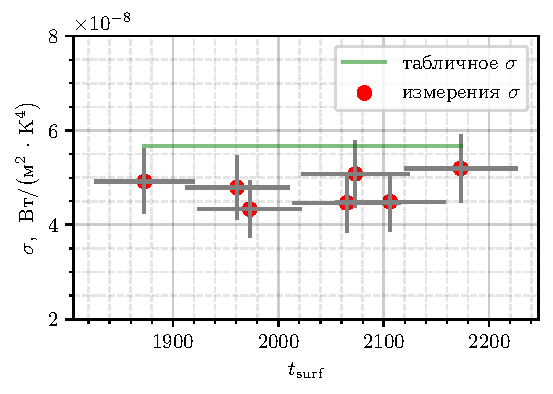
\includegraphics[width=0.5\textwidth]{figs/fig3.pdf}
    \vspace{-5mm}
    \caption{Сравнение полученных значений постоянной Стефана-Больцмана с табличным значением}
    %\label{fig:}
\end{figure}
